% ---------------------------------------------------------------------
% Fixed-cardinality resampling closes the neighbourhood-cardinality
% leak channel. Standalone; compile alone or \input into the paper.
% Requires: \usepackage{tikz} and \usetikzlibrary{arrows.meta,positioning}
% ---------------------------------------------------------------------
\documentclass[tikz,border=4pt]{standalone}
\usepackage{tikz}
\usetikzlibrary{arrows.meta}

\definecolor{evteal}{HTML}{1D9E75}
\definecolor{evtealbg}{HTML}{E1F5EE}
\definecolor{evcoral}{HTML}{D85A30}
\definecolor{evcoralbg}{HTML}{FAECE7}
\definecolor{evgray}{HTML}{888780}
\definecolor{evgraybg}{HTML}{F1EFE8}

\begin{document}
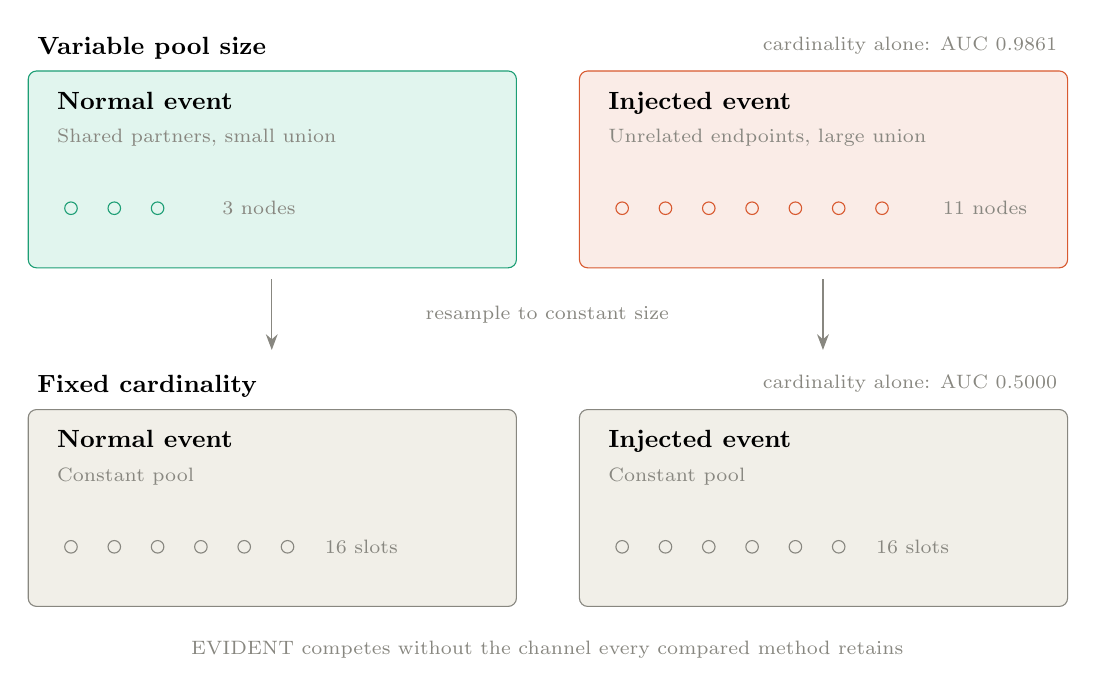
\begin{tikzpicture}[
  font=\small,
  pool/.style={rounded corners=3pt, draw, line width=0.4pt,
               minimum width=6.2cm, minimum height=2.5cm, anchor=north west},
  nd/.style={circle, draw, line width=0.4pt, inner sep=1.6pt},
  ar/.style={-{Stealth[length=2mm]}, line width=0.5pt, draw=evgray}]

% ---- variable cardinality -------------------------------------------
\node[anchor=north west, font=\small\bfseries] at (0,0.55) {Variable pool size};
\node[anchor=north east, font=\scriptsize, text=evgray]
     at (13.2,0.55) {cardinality alone: AUC $0.9861$};

\node[pool, fill=evtealbg, draw=evteal] (nv) at (0,0) {};
\node[anchor=north west, font=\small\bfseries] at (0.25,-0.15) {Normal event};
\node[anchor=north west, font=\scriptsize, text=evgray]
     at (0.25,-0.62) {Shared partners, small union};
\foreach \i in {0,1,2}
  \node[nd, fill=evtealbg, draw=evteal] at (0.55+0.55*\i,-1.75) {};
\node[anchor=west, font=\scriptsize, text=evgray] at (2.35,-1.75) {3 nodes};

\node[pool, fill=evcoralbg, draw=evcoral] (av) at (7,0) {};
\node[anchor=north west, font=\small\bfseries] at (7.25,-0.15) {Injected event};
\node[anchor=north west, font=\scriptsize, text=evgray]
     at (7.25,-0.62) {Unrelated endpoints, large union};
\foreach \i in {0,...,6}
  \node[nd, fill=evcoralbg, draw=evcoral] at (7.55+0.55*\i,-1.75) {};
\node[anchor=west, font=\scriptsize, text=evgray] at (11.5,-1.75) {11 nodes};

% ---- transition ------------------------------------------------------
\draw[ar] (3.1,-2.65) -- (3.1,-3.55);
\draw[ar] (10.1,-2.65) -- (10.1,-3.55);
\node[font=\scriptsize, text=evgray] at (6.6,-3.1) {resample to constant size};

% ---- fixed cardinality ----------------------------------------------
\node[anchor=north west, font=\small\bfseries] at (0,-3.75) {Fixed cardinality};
\node[anchor=north east, font=\scriptsize, text=evgray]
     at (13.2,-3.75) {cardinality alone: AUC $0.5000$};

\node[pool, fill=evgraybg, draw=evgray] (nf) at (0,-4.3) {};
\node[anchor=north west, font=\small\bfseries] at (0.25,-4.45) {Normal event};
\node[anchor=north west, font=\scriptsize, text=evgray]
     at (0.25,-4.92) {Constant pool};
\foreach \i in {0,...,5}
  \node[nd, fill=evgraybg, draw=evgray] at (0.55+0.55*\i,-6.05) {};
\node[anchor=west, font=\scriptsize, text=evgray] at (3.65,-6.05) {16 slots};

\node[pool, fill=evgraybg, draw=evgray] (af) at (7,-4.3) {};
\node[anchor=north west, font=\small\bfseries] at (7.25,-4.45) {Injected event};
\node[anchor=north west, font=\scriptsize, text=evgray]
     at (7.25,-4.92) {Constant pool};
\foreach \i in {0,...,5}
  \node[nd, fill=evgraybg, draw=evgray] at (7.55+0.55*\i,-6.05) {};
\node[anchor=west, font=\scriptsize, text=evgray] at (10.65,-6.05) {16 slots};

\node[font=\scriptsize, text=evgray] at (6.6,-7.35)
  {EVIDENT competes without the channel every compared method retains};
\end{tikzpicture}
\end{document}
